
\documentclass{article}
\usepackage[margin=1in]{geometry}
\usepackage{amsmath}
\usepackage{graphicx}
\begin{document}

\section*{Computational Biology Bootcamp Assignment: Permutation Test for Correlation}
Author : Anna Cavalieri Canosa}

\section*{Introduction and Methodology}
The \emph {KeyWestAnnualMeanTemperature} dataset was analysed in R using Visual Studio Code. 
A permutation test was carried out to evaulate the correlation between years and temperature. 
The test involved 10000 random shuffles of the temperature data to assess the likelihood of observing the correlation by chance.

\section*{Results and Conclusion}
The observed correlation coefficient was $r = 0.533$, indicating a moderate positive relationship between years and temperature. 
This suggests that, on average, temperatures have increased over time. This relationship was found to be statistically significant.
as the p-value obtained was $p = 0$. The null hypothesis was therefore rejected.. 
This outcome indicates that the observed correlation is highly unlikely to be due to random chance. 
Figure 1 below illustrates the distribution of random correlation coefficients obtained from the permutation test. 
The observed correlation is represented by a red dashed line, which is absent in the figure. This absence highlights the extremity of the observed correlation and reinforces its statistical significance. 


\begin{figure}[h!]
\centering
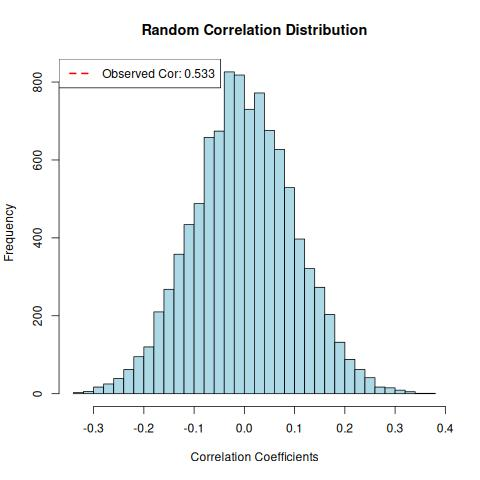
\includegraphics[height = 0.6\textwidth]{../results/random_correlation_hist.jpg}
\caption{Histogram of random correlation coefficients from the permutation test.}
\label{fig:random_corr_hist}
\end{figure}


\end{document}

